\documentclass[twoside,11pt]{article}

% Any additional packages needed should be included after jmlr2e.
% Note that jmlr2e.sty includes epsfig, amssymb, natbib and graphicx,
% and defines many common macros, such as 'proof' and 'example'.
%
% It also sets the bibliographystyle to plainnat; for more information on
% natbib citation styles, see the natbib documentation, a copy of which
% is archived at http://www.jmlr.org/format/natbib.pdf

\usepackage{jmlr2e}
\usepackage{lipsum}
\usepackage{amsmath}
\usepackage{hyperref}
\usepackage{algorithm,algorithmic}
\usepackage{soul} % highlight
\usepackage{xcolor}
\usepackage{listings}
\usepackage[normalem]{ulem}

\lstdefinestyle{mystyle}{
    backgroundcolor=\color{gray!5},        % Very very light gray background
    basicstyle=\ttfamily\scriptsize,      % Typewriter font with smaller size
    commentstyle=\color{gray},            % Comment color
    keywordstyle=\color{blue},            % Keyword color
    stringstyle=\color{red},              % String color
    breaklines=true,                      % Automatically break long lines
    frame=single,                         % Draw a frame around the code
    rulecolor=\color{lightgray},          % Frame color set to light gray
    showspaces=false,                     % Don't show spaces
    showstringspaces=false,               % Don't show spaces in strings
    showtabs=false,                       % Don't show tabs
    tabsize=4                             % Set default tab size
}

\setcitestyle{square}

% Definitions of handy macros can go here

\newcommand{\dataset}{{\cal D}}
\newcommand{\fracpartial}[2]{\frac{\partial #1}{\partial  #2}}

\renewcommand{\algorithmicrequire}{\textbf{Input:}}
\renewcommand{\algorithmicensure}{\textbf{Output:}}

\makeatletter
\renewcommand\subsubsection{\@startsection{subsubsection}{3}{\z@}%
  {-3.25ex\@plus -1ex \@minus -.2ex}%
  {1.5ex \@plus .2ex}%
  {\normalfont\bfseries\normalsize}}
\makeatother

% Heading arguments are {volume}{year}{pages}{submitted}{published}{author-full-names}
\jmlrheading{}{2024}{}{}{}{Griffon, Smoliakov, Yntykbay}

% Short headings should be running head and authors last names

\ShortHeadings{Predicting Air Pollution Levels in India}{Griffon, Smoliakov, Yntykbay}
\firstpageno{1}

\begin{document}

\title{Predicting Air Pollution Levels in Five Major Indian Cities}

\author{\name Aleksandr Jan Smoliakov \email aleksandr.smoliakov@mif.stud.vu.lt \\
  \name Danial Yntykbay \email danial.yntykbay@mif.stud.vu.lt \\
  \name Davide Giuseppe Griffon \email davide.griffon@mif.stud.vu.lt \\
  \addr Data Science study programme\\
       Faculty of Mathematics and Informatics}

\editor{Jurgita Markevi\v{c}i\={u}t\.{e}}

\maketitle


\begin{abstract}

  Air pollution ranks among the most pressing global health threats, causing an estimated 3 to 9 million deaths annually.
  India, with its rapid urbanization and economic growth, faces some of the highest pollution levels globally. The country's air pollution stems from a combination of natural and anthropogenic sources, emitting harmful pollutants such as carbon monoxide (CO) and particulate matter (PM\textsubscript{10} and PM\textsubscript{2.5}).

  This project aims to develop a predictive model for air pollution levels using a multivariate regression approach. The model will incorporate a wide array of predictors, including geographic location, seasonal variations, meteorological data and temperature. By evaluating various modeling techniques—starting with linear regression and potentially expanding to more complex methods such as Random Forest—and analyzing data correlations, the study seeks to identify the most effective methods for accurately forecasting urban air pollution levels.
  
  This topic was chosen due to its relevance in addressing the escalating air quality issues in India and the availability of extensive historical weather and air quality data. Previous studies on air quality prediction often focus on pollutants like PM\textsubscript{2.5} and PM\textsubscript{10}. Here, we broaden the scope by analyzing seven different pollutants across five major Indian cities—Bengaluru (Bangalore), Delhi, Hyderabad, Jaipur, and Mumbai—assessing their seasonal trends and interdependencies, and examining a wider set of meteorological and temporal variables. The study also enhances interpretability by comparing feature importance across cities, offering a clearer understanding of regional differences.
  
  This study will demonstrate the practical application of data mining techniques using real-world environmental data, serving as a foundation for further exploration in this field.
  
\end{abstract}

\newpage



% ---------------------------------------------------------------------------------------
% ---------------------------------------------------------------------------------------
% ---------------------------------------------------------------------------------------



\section{Literature Review}
Air pollution has been extensively studied worldwide due to its significant impacts on public health, ecosystems, and the economy. Numerous studies have demonstrated the adverse health effects of air pollutants, including respiratory and cardiovascular diseases, leading to increased morbidity and mortality rates. Particularly, countries like India and China have received considerable attention because of their severe air quality issues, which are exacerbated by rapid industrialization, urbanization, and population growth.

During our literature review, we encountered a vast number of articles related to our research topic. The widespread interest among scientists and data analysts facilitated the collection of numerous sources. As our research progressed, we found that many studies have attempted to develop statistical and artificial intelligence models to predict air pollution levels, utilizing both global datasets and data specific to particular regions. Researchers have employed a variety of techniques, including multivariate regression, neural networks, and machine learning algorithms, to forecast pollutant concentrations based on diverse predictors such as meteorological conditions, emission sources, and socio-economic factors. These models have been applied at various regional scales, providing valuable insights for environmental management and policy-making. Despite this extensive body of research providing a solid foundation for our study, we have not found any existing studies that have examined the five major Indian cities using the same datasets we are using in this project.

To effectively manage and synthesize the extensive body of literature, we have chosen not to include general studies on air pollution in India, as they do not directly contribute to the development of our predictive model. Instead, we have focused our review on two specific categories of research that are more pertinent to our objectives: "Causal and Correlational Studies on Urban Air Pollution" and "Predictive Models". The first category delves into the factors influencing air pollution levels in urban areas, providing valuable insights that inform the selection of variables and the structural framework of our model. The second category encompasses studies that have developed predictive models for air pollution, offering methodologies and approaches that we can build upon to enhance the accuracy and reliability of our own model. By concentrating on these two groups, we aim to leverage existing knowledge effectively and advance our research in a meaningful way.

\subsection{Causal and Correlational Studies on Urban Air Pollution}

Understanding the dynamics of urban air pollution is essential for developing effective strategies to enhance air quality and protect public health. Several studies have focused on analyzing the correlations and underlying causes of air pollution in metropolitan environments, rather than constructing predictive models.

For instance, \citep{refId0} conducted a six-year analysis in Pune, India, assessing the correlations between pollutants and meteorological factors. The study revealed that most pollutants were positively correlated with each other and with temperature, except for O\textsubscript{3}, which had a negative correlation. Wind speed showed a strong negative correlation with pollutant levels, emphasizing its role in pollutant dispersion.

Building on similar themes, \citep{M2024AirQuality} investigated air pollution across various urban hotspots in Chennai, India. This research assessed hourly concentrations of pollutants such as PM\textsubscript{10}, PM\textsubscript{2.5}, SO\textsubscript{2}, NO\textsubscript{2}, and CO across key areas—industrial, traffic, commercial, and residential zones—over the course of 2022. A key methodological approach employed in this study is the Coefficient of Divergence (COD), which quantifies spatial variations in pollutant concentrations among the different hotspots. One of the significant findings of the Chennai study is the impact of wind on pollution dispersion. When wind speeds are low (0–3 m/s), CO levels tend to be higher, indicating that pollutants are not dispersing effectively and are accumulating near their sources. Conversely, when the wind blows from the south and southeast at moderate speeds (2–6 m/s), the concentrations of PM\textsubscript{2.5} and PM\textsubscript{10} increase. This suggests that pollutants from nearby industries are being transported toward the monitoring stations, highlighting the crucial role of meteorological conditions in air quality.

In another study, \citep{Suthar2024Annual} aimed to identify seasonal patterns and understand how meteorological factors influence pollutant levels in a different Indian city. The research included a correlation analysis between air pollutants and meteorological parameters—wind speed (WS), wind direction (WD), relative humidity (RH), and solar radiation (SR). Over three consecutive years, the analysis revealed that WD, WS, and RH generally had a negative correlation with all measured air pollutants. Calm wind conditions inhibit the dispersion of pollutants, resulting in higher concentrations near the ground, underscoring the importance of WS and WD in the dispersion and transport of air pollutants.

Expanding this line of research to European cities, \citep{Rowland2024} examined the relationship between meteorological parameters and the concentrations of NO\textsubscript{2}, O\textsubscript{3}, PM\textsubscript{10}, and PM\textsubscript{2.5} in Krakow, Paris, and Milan during 2021. The study found that NO\textsubscript{2}, PM\textsubscript{10}, and PM\textsubscript{2.5} concentrations were higher during winter and lower during summer, exhibiting negative correlations with temperature, while O\textsubscript{3} showed the opposite trend. Wind speed was inversely related to particulate matter and NO\textsubscript{2} levels but positively correlated with O\textsubscript{3} concentrations. These findings highlight the influence of meteorological conditions on pollutant levels and the occurrence of the “Ozone weekend effect” in these cities.

Speaking of temporal trends, \citep{bozhkova2020influence} conducted research in urban areas of Belarus. Seasonal patterns revealed higher pollution in autumn and winter, with increased dispersion of pollutants and ozone formation in spring and summer. The study observed daily pollution peaks occurring in the morning and evening, driven by human activities and affected by wind and atmospheric stability. The reduced dispersion efficiency during these periods, combined with higher emission intensities, contributes to these peaks.

These studies collectively underscore the significant impact of meteorological and temporal factors on urban air pollution across diverse geographic regions. The consistent observations of pollutant behavior in relation to temperature, wind speed, and other meteorological parameters highlight the necessity of incorporating environmental conditions into air quality management and policy-making.


\subsection{Predictive Models}

Predictive modeling plays a crucial role in understanding and forecasting air pollution levels, which is essential for public health planning and environmental management. Various studies have employed different statistical and machine learning approaches to predict concentrations of air pollutants and the Air Quality Index (AQI), a standardized measure that indicates the overall air quality and its potential impact on human health.

Singh et al.\ \citep{SINGH2012244} investigated both linear and nonlinear methods for forecasting urban air quality, aiming to improve prediction accuracy in complex urban environments. The study examined the effectiveness of different modeling approaches for predicting concentrations of common urban pollutants such as PM$_{10}$, NO, CO, and O$_3$. Specifically, they applied linear models like multiple linear regression and nonlinear models including Artificial Neural Networks (ANNs) to compare their performance in capturing pollution patterns. The findings indicated that nonlinear models, particularly ANNs, provided better prediction accuracy than linear models, highlighting the importance of nonlinear approaches in modeling air pollution in urban settings.

Sanjeev et al.\ \citep{Sanjeev2021} developed predictive models for air quality using machine learning algorithms, focusing on Artificial Neural Networks (ANN), Support Vector Machines (SVM), and Random Forests (RF). Their study aimed to identify the most efficient algorithm for air quality prediction. The models were evaluated based on accuracy scores, with the RF-based model achieving the highest accuracy.

Kothandaraman et al.\ \citep{Kothandaraman2022Intelligent} focused on predicting PM${2.5}$ pollutant levels by employing a variety of machine learning algorithms, including linear regression, Random Forest, K-Nearest Neighbors, Ridge and Lasso regression, XGBoost, and AdaBoost. Their study utilized historical PM${2.5}$ data and relevant meteorological features such as temperature, humidity, wind speed, and precipitation collected from monitoring stations in Anand Vihar, Delhi, over the period from January 2014 to December 2019. By evaluating the performance of these models through statistical metrics like Mean Absolute Error (MAE), Root Mean Square Error (RMSE), and R-squared ($R^2$), they found that ensemble methods such as XGBoost and Random Forest outperformed other algorithms in terms of predictive accuracy. These results highlight the effectiveness of advanced machine learning techniques in modeling air pollution and the critical role of incorporating meteorological data.

Kumar et al.\ \citep{Kumar2023} addressed the challenge of predicting the AQI by analyzing air pollution data from 23 Indian cities over six years. They carried out extensive data preprocessing, which involved handling missing values, correcting outliers, normalizing data, selecting features, and applying logarithmic transformations to fix skewed data. Their exploratory data analysis showed a significant decrease in pollution levels in 2020, likely due to COVID-19 lockdowns. To fix data imbalance, they used the Synthetic Minority Over-sampling Technique (SMOTE). They performed machine learning-based AQI predictions using various models, both with and without SMOTE resampling, and compared the results. The models were assessed using standard metrics like accuracy, precision, recall, F1-score, and error metrics (MAE, RMSE, RMSLE, $R^2$). The XGBoost model performed the best, achieving the highest accuracy in both training and testing phases, while the SVM model had the lowest accuracy. The Random Forest model also did well, especially when SMOTE was applied. The study emphasizes the effectiveness of ensemble learning methods in AQI prediction and suggests that future research could explore deep learning techniques to improve accuracy further.

Roy et al.\ \citep{ROY20244106} conducted a study in the densely populated northern Indian states of Delhi, Haryana, and Uttar Pradesh, analyzing PM${2.5}$ concentrations in relation to meteorological factors such as temperature, precipitation, surface pressure, and wind. They employed Ordinary Least Squares (OLS) regression and Geographically Weighted Regression (GWR) to explore the relationships between PM${2.5}$ levels and environmental parameters across different seasons and locations. The OLS model identified significant predictors with $R^2$ values of 0.93 for summer and 0.94 for winter, while GWR accounted for spatial variability, enhancing model performance and highlighting the importance of geographical factors in air pollution modeling. However, our study does not utilize geographical data and cannot replicate the GWR analysis by Roy et al. Instead, we focus on the overall relationships between PM${2.5}$ concentrations and meteorological factors without considering spatial variability.

Building on the significance of feature engineering and advanced modeling techniques, \citep{naz2024twostage} emphasized the crucial role of feature engineering in time series prediction of air pollutants. They introduced a two-stage feature engineering and selection process that combines correlation-based selection with Variational Mode Decomposition (VMD). By developing and categorizing 22 new features into meteorological, temporal, statistical, and air pollutant types, their approach customizes optimal feature sets for each of the five major air pollutants. This customization enhances model performance by 1–5\% compared to traditional lag-based methods and further improves accuracy by 3–13\% when integrating VMD features. The optimized feature selection allows for simpler forecasting models with significant improvements in RMSE, MAE, and R\textsuperscript{2} scores.

These studies demonstrate the effectiveness of various machine learning and statistical methods in predicting air pollution levels and AQI. Nonlinear models and ensemble learning techniques like Random Forest and XGBoost have shown high accuracy in forecasting pollutant concentrations and AQI. The incorporation of meteorological and temporal data significantly enhances model performance. For our study, which does not employ deep learning methods, these findings suggest that ensemble methods and regression techniques—especially those accounting for spatial variability—can serve as effective alternatives for accurate air quality prediction. Incorporating meteorological factors and addressing data imbalances may further improve prediction accuracy without the need for deep learning models.

\newpage



% ---------------------------------------------------------------------------------------
% ---------------------------------------------------------------------------------------
% ---------------------------------------------------------------------------------------



\section{Exploratory Data Analysis}

\subsection{Data Source}

This project used two primary sources of data to analyze air pollution levels across five major Indian cities:

\begin{itemize}
    \item \textbf{Air Quality Data in India}: Available at \href{https://www.kaggle.com/datasets/rohanrao/air-quality-data-in-india}{\uline{Kaggle}}. This dataset provides hourly measurements of various air pollutants and particulate matter. The data is collected from multiple weather stations located in 27 major Indian cities. The date range spans from January 2015 to July 2020, with over 700,000 records.

    \item \textbf{Historical Weather Data for Indian Cities}: Available at \href{https://www.kaggle.com/datasets/hiteshsoneji/historical-weather-data-for-indian-cities}{\uline{Kaggle}}. This dataset includes hourly weather-related features across 8 Indian cities, encompassing over 20 variables such as precipitation (mm), wind speed, temperature, humidity, and other meteorological parameters. The date range of the dataset spans from 2006 to 2019, with over 700,000 records. \citep{hitesh_soneji_2020}
\end{itemize}

To extract meaningful insights, it was necessary to merge these datasets, linking the meteorological variables from the second dataset with the air quality measurements from the first. This integration allowed us to analyze how environmental factors such as temperature, wind speed, and precipitation interact with pollutant concentrations over time. The merging process focused on aligning data by city names and hourly timestamps, ensuring that weather features corresponded accurately to pollution levels. This alignment was essential for preserving the temporal and spatial consistency of our analysis. While the original datasets contained information for additional cities and years, we focused our analysis on the five metropolitan areas and the five-year period (January 2015 to January 2019), where the two datasets overlapped.

Looking ahead to our modeling approach, we envisioned using the rich meteorological data, combined with temporal features (such as hour of day and month of year) and the city names as predictors for air quality data.

Note that we will not be forecasting time series data in this project, as we are limited in the choice of models and may not use advanced techniques like LSTM or other deep learning models. Instead, our primary goal is to predict air pollution levels using a multivariate regression approach. This will allow us to explore how various environmental and temporal variables contribute to air pollution patterns and potentially forecast air quality from meteorological data.

In the following subsections, we first examine our response variables, analyzing the various pollutants and their distributions in our dataset. We then explore the weather features, detailing how we identified the most relevant predictors from our merged dataset. Finally, we present our feature engineering methodology, which helped us capture complex temporal and spatial patterns in our data, setting the stage for our subsequent modeling efforts.


\subsection{Response Variable Selection}

The pollution dataset contained twelve potential response variables measuring different air quality parameters: PM\textsubscript{2.5}, PM\textsubscript{10}, NO, NO\textsubscript{2}, NOx, NH\textsubscript{3}, CO, SO\textsubscript{2}, O\textsubscript{3}, Benzene, Toluene, and Xylene. While we initially considered calculating and using the Air Quality Index (AQI) as a comprehensive response variable, this approach proved impractical due to the dataset's structure. The AQI calculation requires complete data across multiple pollutants, and the presence of missing values in our dataset would have significantly limited our ability to compute this index accurately.

After careful consideration of data completeness and relevance, we narrowed our focus to seven key pollutants that demonstrated the most complete records: PM\textsubscript{2.5}, PM\textsubscript{10}, NOx, NH\textsubscript{3}, CO, SO\textsubscript{2}, and O\textsubscript{3}. The analysis of missing data revealed varying degrees of incompleteness across these pollutants, with CO showing the lowest proportion at 4\% missing values, followed by NOx at 9\%, SO\textsubscript{2} at 19\%, PM\textsubscript{2.5} and O\textsubscript{3} both at approximately 20\%, PM\textsubscript{10} at 26\%, and NH\textsubscript{3} showing the highest proportion at 30\% missing values.

To maintain data integrity and avoid potential biases, we chose to handle missing values through complete case deletion rather than imputation. This decision was supported by the large volume of available data in our merged dataset, which allowed us to maintain a robust sample size even after removing incomplete records. We applied this deletion approach consistently across both air quality parameters and meteorological features to ensure data consistency.

\subsubsection{Distribution Analysis and Transformation}

Initial exploratory analysis revealed that the distributions of these pollutants exhibited strongly right-skewed patterns across all five cities. Figure~\ref{fig:skewness} illustrates this pattern for three representative pollutants, but the same asymmetric distribution was observed across all pollutants, characterized by a high frequency of lower values and a long tail extending toward higher concentrations.

\begin{figure}[H]
  \centering
  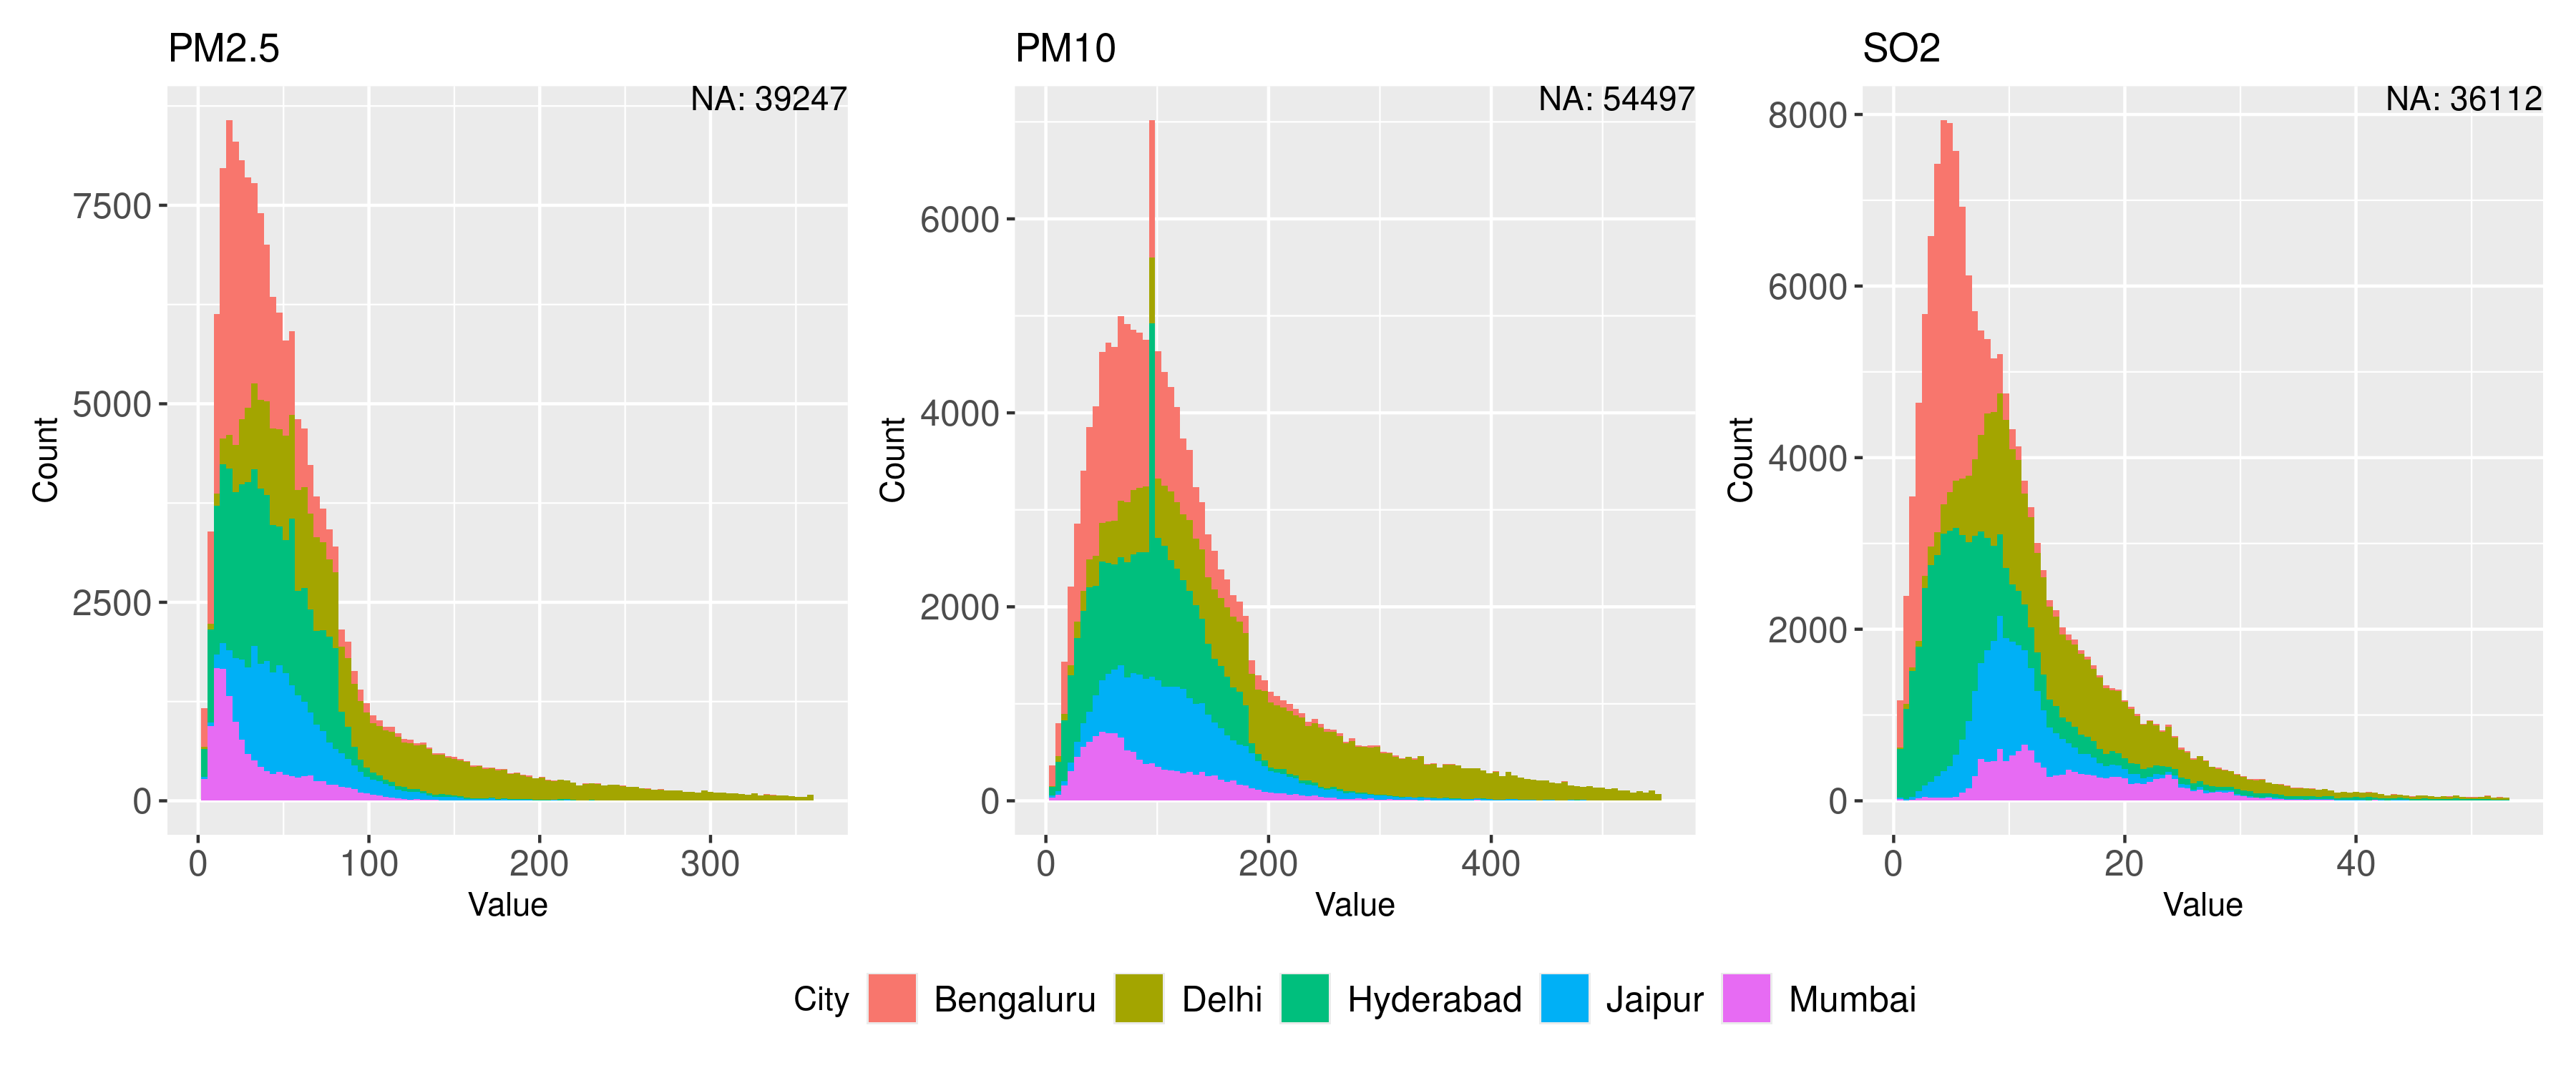
\includegraphics[width=\textwidth]{assets/skewness.png}
  \caption{Pollutants levels by city}
  \label{fig:skewness}
\end{figure}

To address this skewness and make the data more suitable for statistical analysis, we applied a logarithmic transformation to all pollutant measurements. Since logarithmic transformation requires strictly positive values, we added a constant of 1 to each measurement before applying the transformation. The effectiveness of this transformation is demonstrated in Figure~\ref{fig:log_scaled_pollutants}, where the transformed distributions more closely approximate normal distributions, providing a more suitable basis for our subsequent analyses.

\begin{figure}[H]
  \centering
  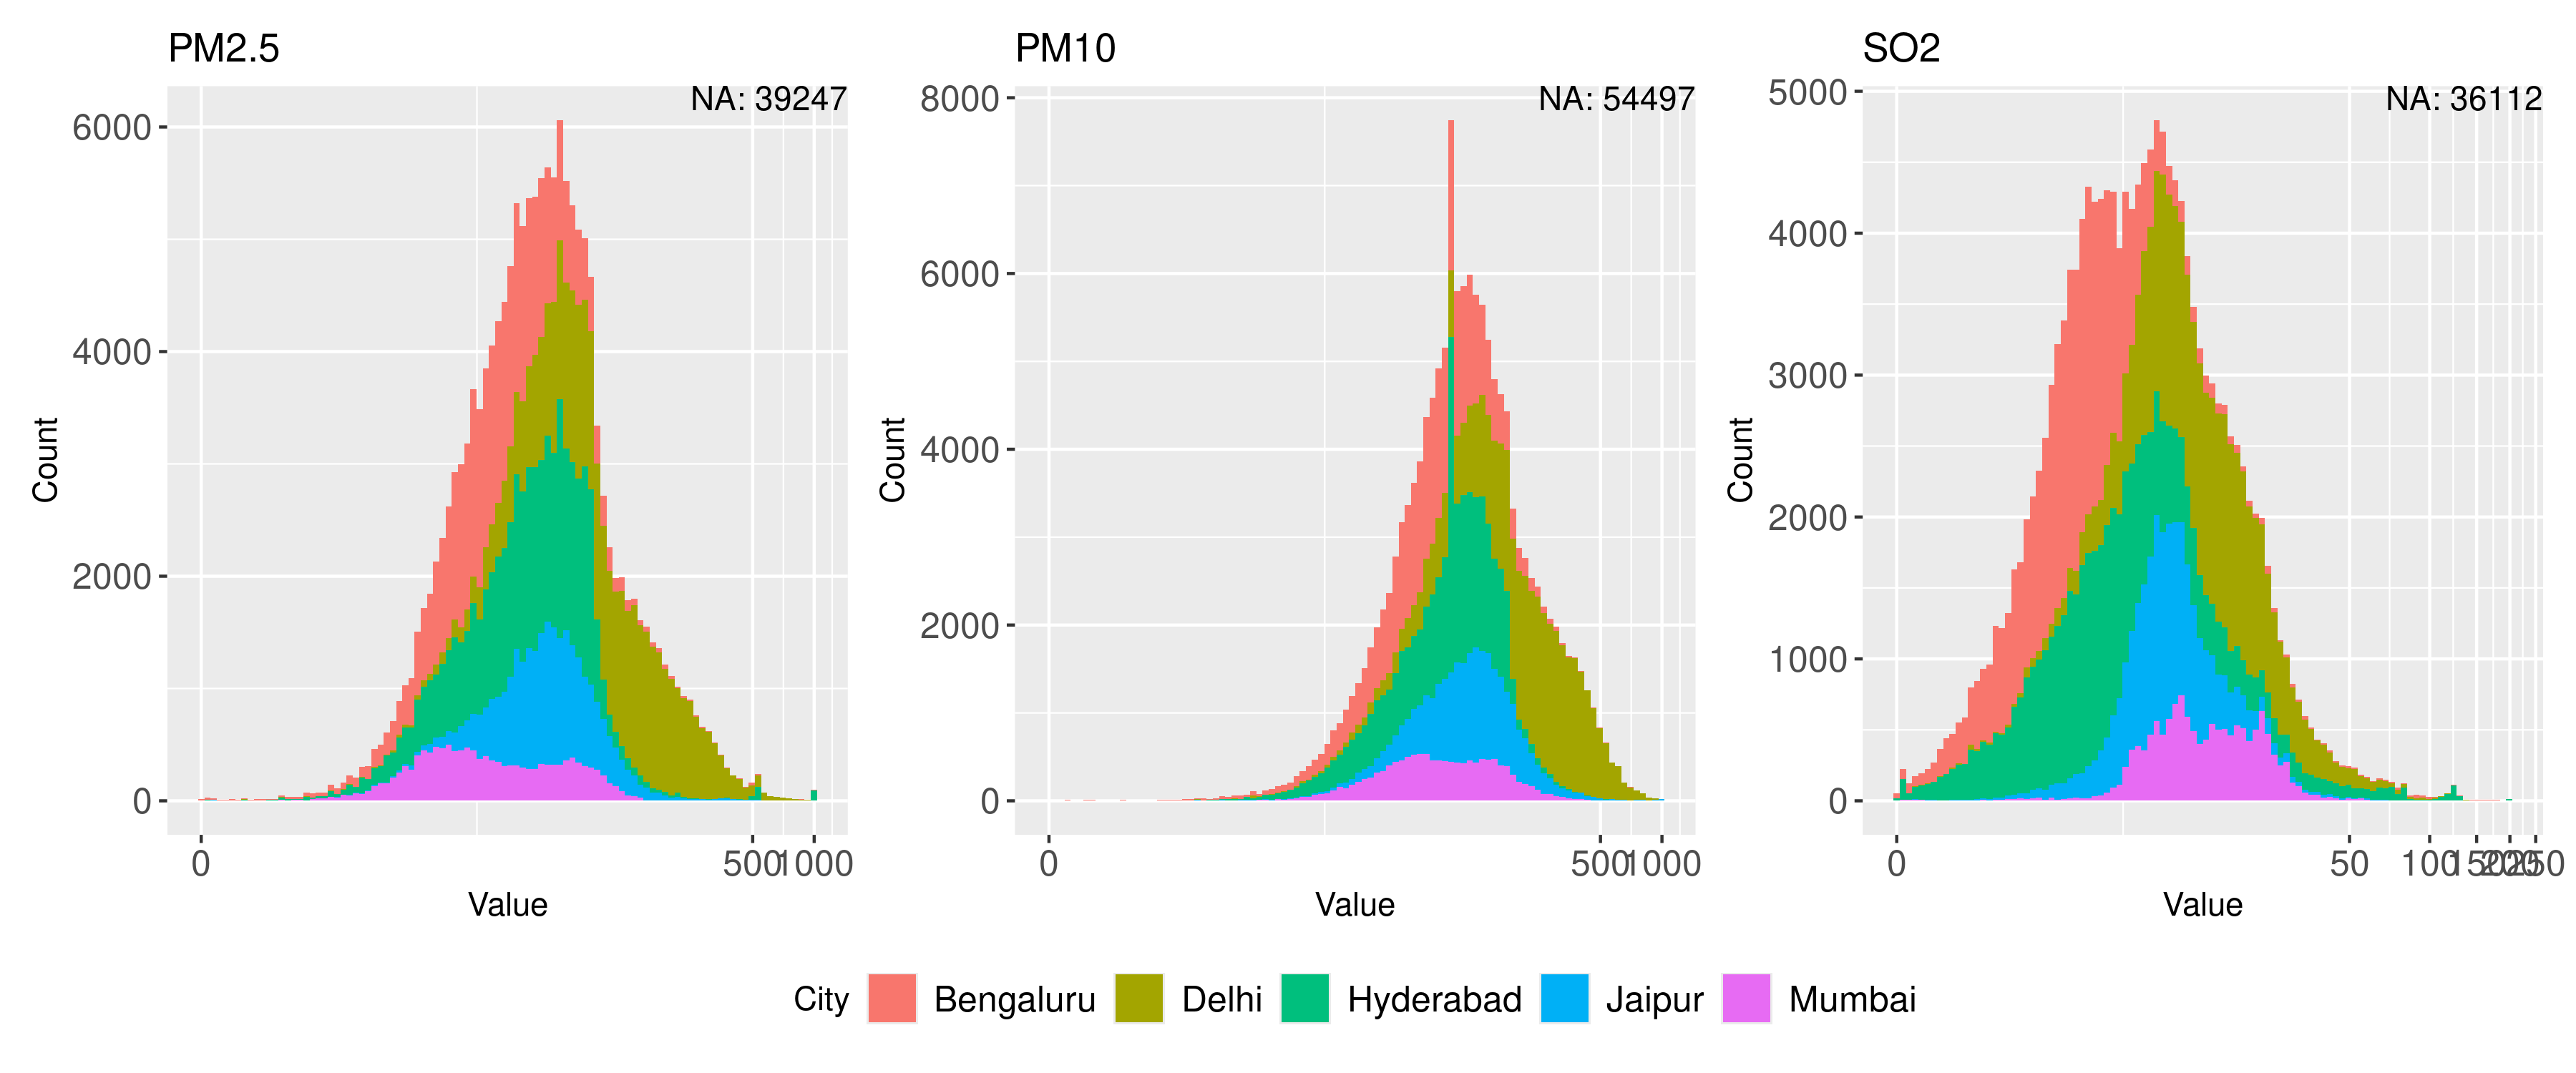
\includegraphics[width=\textwidth]{assets/log-scaled-pollutants.png}
  \caption{Pollutants levels by city on a logarithmic scale}
  \label{fig:log_scaled_pollutants}
\end{figure}

\subsubsection{Temporal Pattern Analysis}

Further investigation of temporal patterns revealed distinct seasonal trends in pollutant concentrations, particularly for PM\textsubscript{2.5} and PM\textsubscript{10}, as shown in Figure~\ref{fig:seasonal_trends}. Notable patterns can be observed for PM\textsubscript{2.5} and PM\textsubscript{10}, where consistently lower concentrations were observed across all cities. Among the cities studied, Delhi consistently exhibited higher pollutant concentrations throughout the year. These temporal patterns suggest the importance of incorporating seasonal factors into our modeling approach. While there are clear seasonal trends in the data, they do not always follow a simple sinusoidal pattern, and the minimums are observed at different times of the year for different pollutants.

All this complexity suggests that different cities should be modeled separately, and the seasonal trends may require more sophisticated modeling techniques to capture accurately.

\begin{figure}[H]
  \centering
  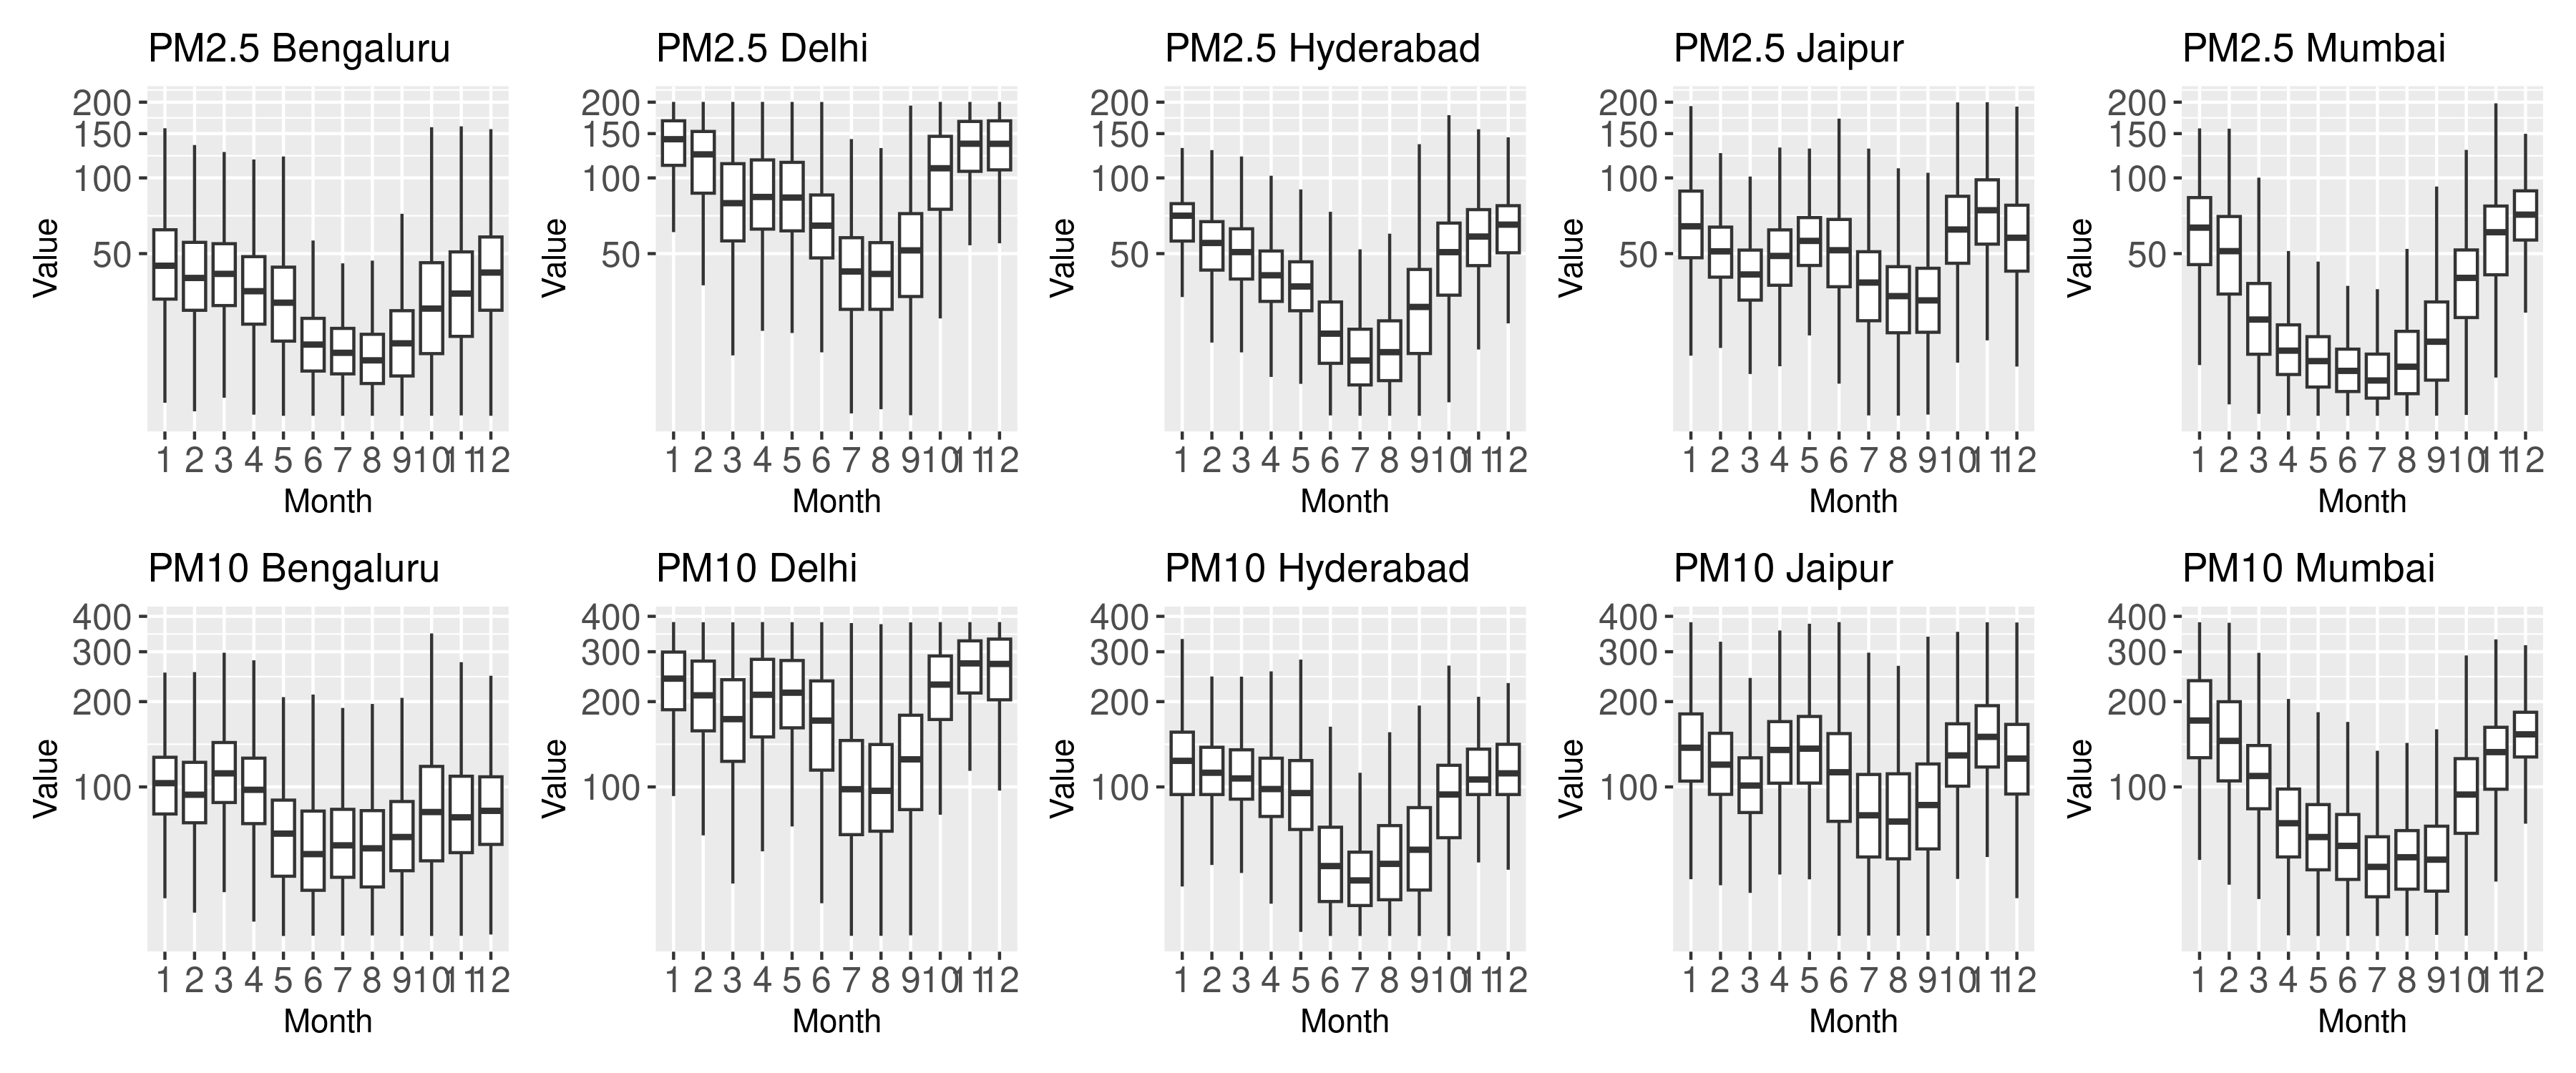
\includegraphics[width=\textwidth]{assets/seasonal-trends.png}
  \caption{Monthly PM\textsubscript{2.5} and PM\textsubscript{10} distributions by city}
  \label{fig:seasonal_trends}
\end{figure}

\subsection{Predictor Selection}

Having completed our analysis of the pollutant response variables and their distributions, we turned our attention to examining the meteorological predictors in our dataset. Before applying feature selection, we conducted a correlation analysis of the meteorological data to understand the relationships between weather variables. The correlation matrix visualization (Figure~\ref{fig:correlation_matrix}) revealed several significant relationships between weather parameters. Some of the key findings were as follows:

\begin{figure}[H]
  \centering
  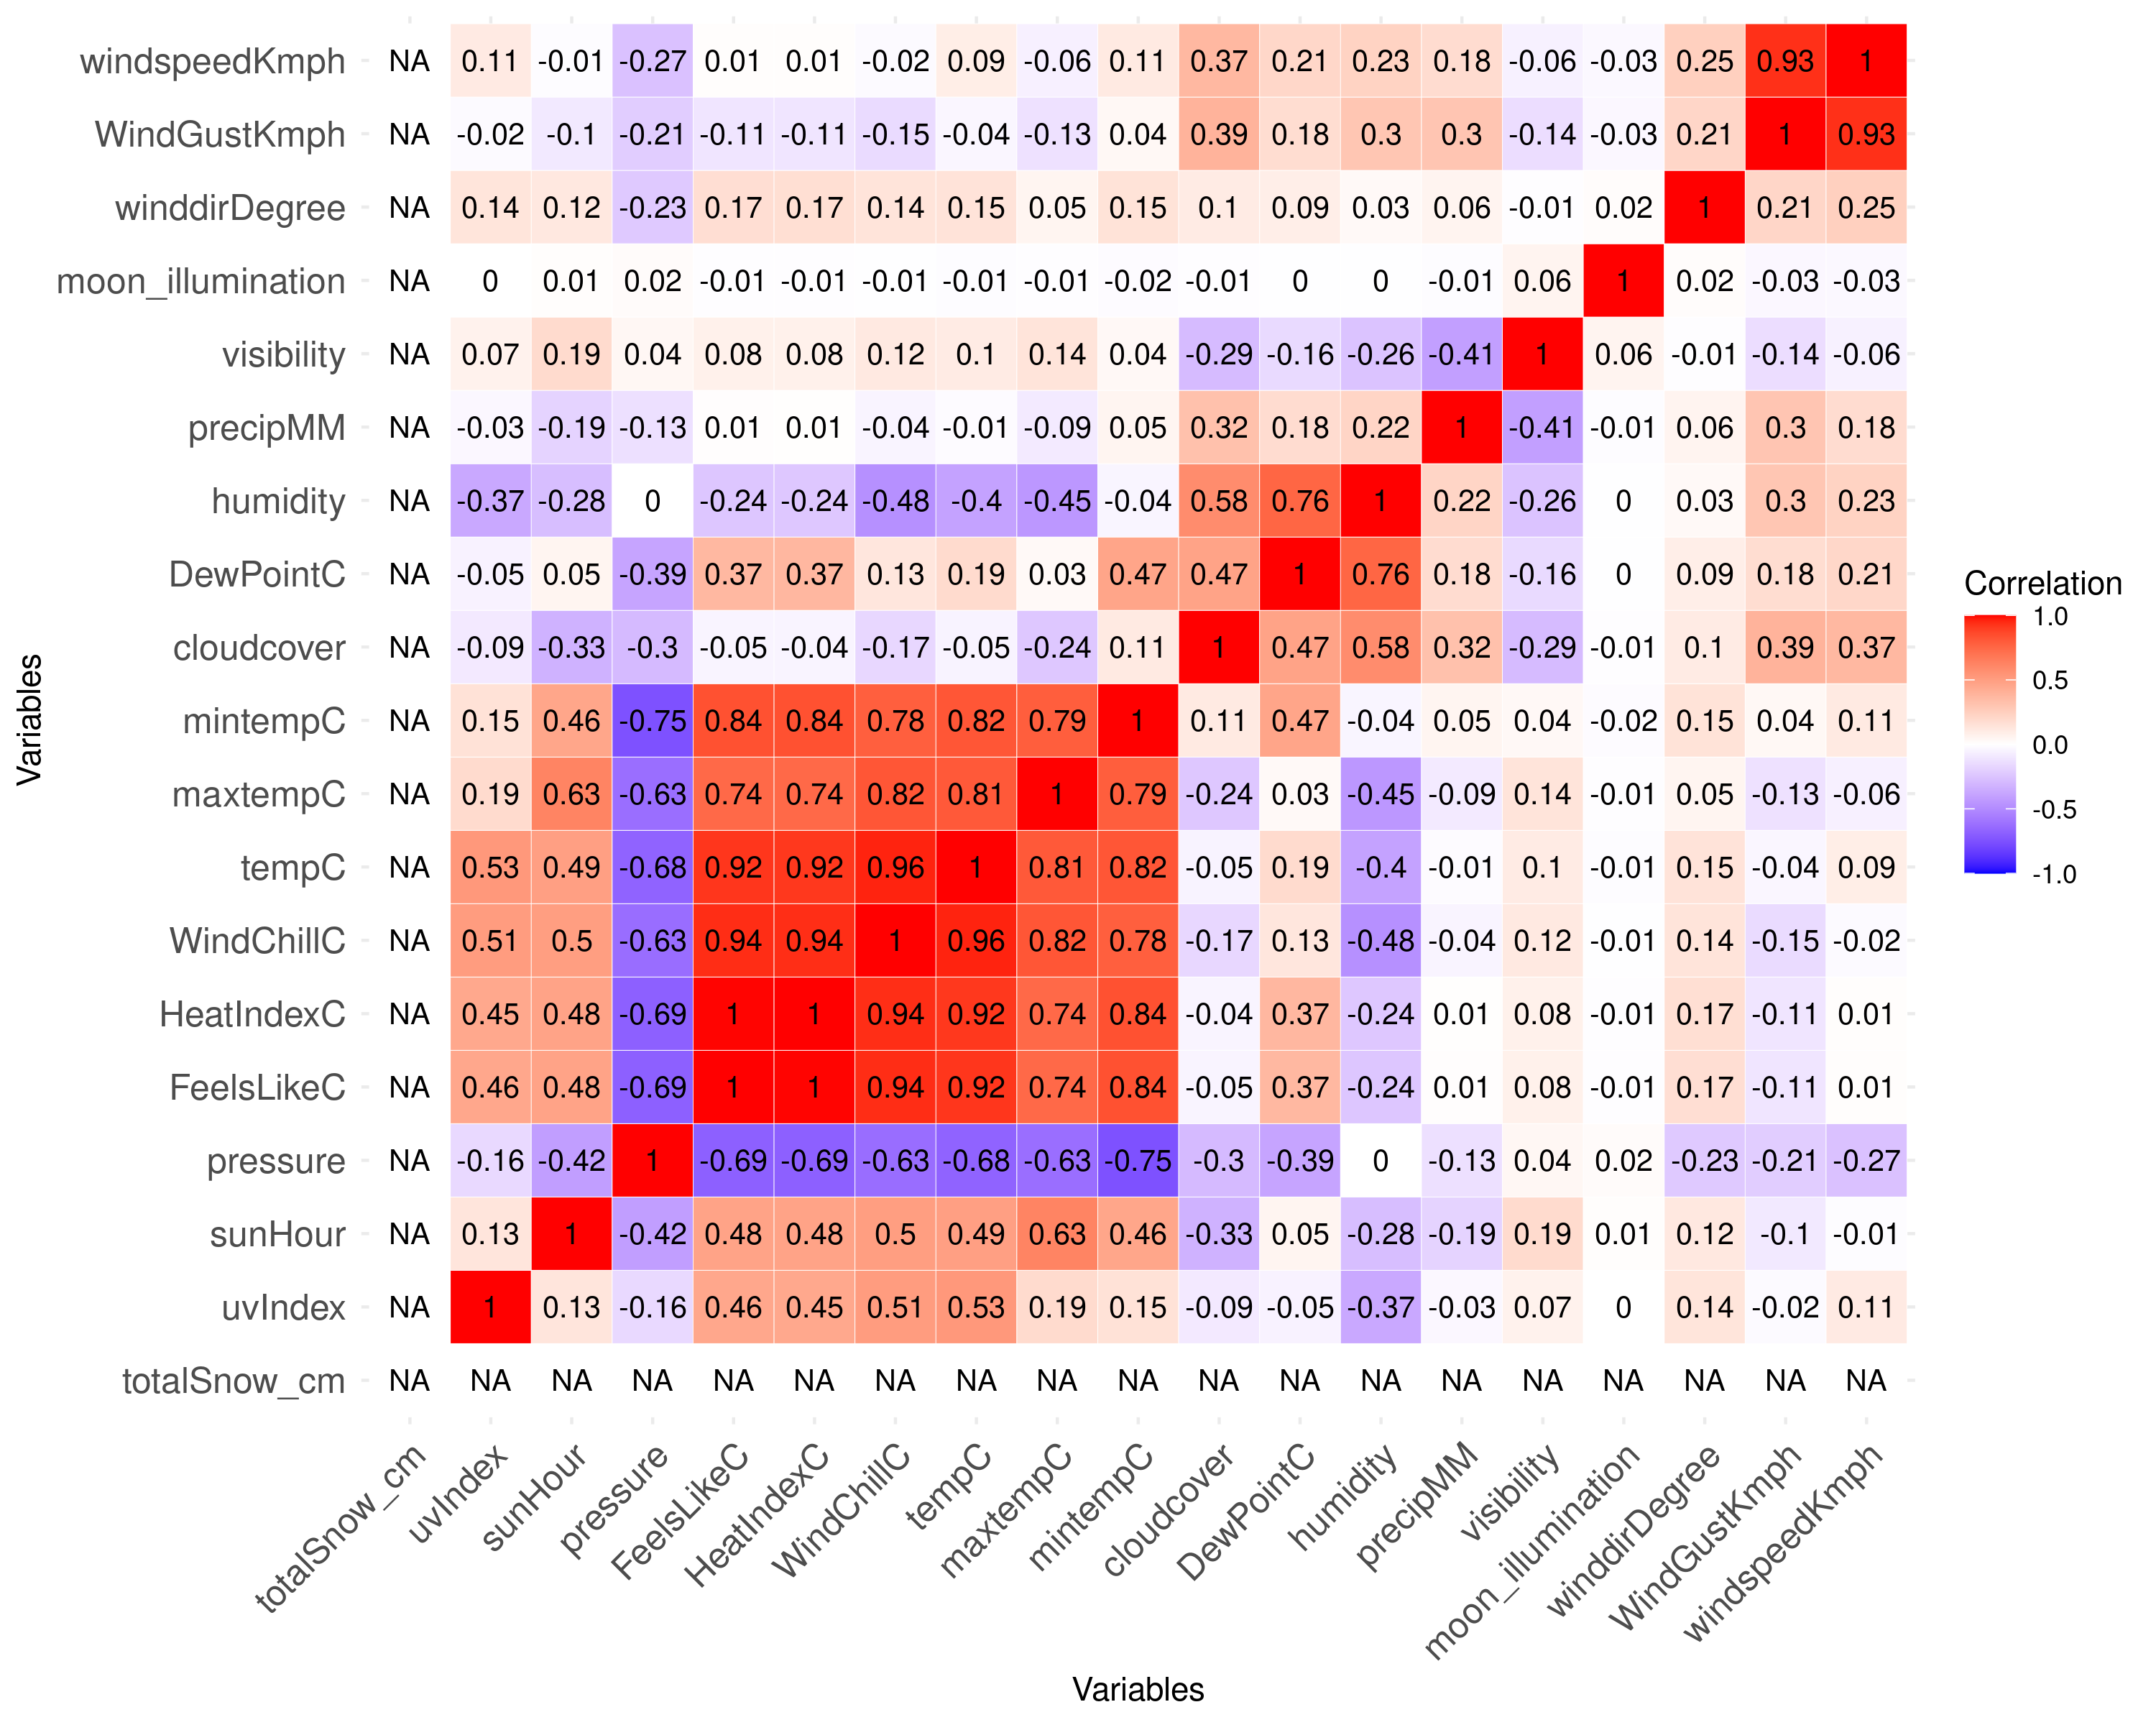
\includegraphics[width=\textwidth]{assets/feature-correlation-matrix.png}
  \caption{Correlation matrix of weather variables.}
  \label{fig:correlation_matrix}
\end{figure}

\begin{itemize}
    \item \textit{FeelsLikeC}, \textit{HeatIndexC}, \textit{WindChillC}, \textit{minTempC}, and \textit{maxTempC} were very strongly correlated with \textit{tempC}, as expected, given that they are derived from temperature, humidity, and wind speed.
    \item Features like \textit{sunHour} and \textit{uvIndex} were also correlated with temperature-related variables.
    \item \textit{Humidity} was positively correlated with \textit{DewPointC} and \textit{cloudcover}, while inversely correlated with temperature-related variables.
    \item \textit{Pressure} was inversely correlated with temperature-related variables and showed slight correlations with several other features, suggesting that pressure is influenced by other meteorological factors.
    \item \textit{Visibility} exhibited slight positive correlations with temperature-related variables and inverse correlations with \textit{humidity}, \textit{cloudcover}, \textit{precipitation}, and \textit{DewPointC}.
    \item \textit{Windspeed} and \textit{windgust} were strongly correlated with each other.
    \item \textit{Moon\_illumination} was not correlated with any other variable, as expected.
\end{itemize}

Based on these findings, we identified several highly correlated group of features, such as \textit{tempC} and \textit{FeelsLikeC}, \textit{HeatIndexC}, and \textit{WindChillC}, which could potentially introduce collinearity issues in our models. To address this, we have removed the highly correlated features, retaining only one representative variable from each correlated pair. This feature selection process aimed to reduce redundancy and improve model interpretability by focusing on the most relevant predictors. The following predictors were removed from our dataset:

\begin{itemize}
    \item \textit{totalSnow\_cm} was removed due to zero variance.
    \item \textit{FeelsLikeC}, \textit{HeatIndexC}, and \textit{WindChillC} were removed in favor of \textit{tempC}.
    \item \textit{WindGustKmph} was removed in favor of \textit{windspeedKmph}.
    \item \textit{Visibility} was removed due to it being a possible leakage feature.
    % \item \textit{minTempC} and \textit{maxTempC} were removed in favor of \textit{tempC}.
\end{itemize}

Following this, we analyzed the correlation between the selected features (those obtained after removing the highly correlated ones identified in the previous analysis) and the response variables to assess their potential predictive power. The resulting correlation analysis is visualized in Figure~\ref{fig:feature_response_correlation}.

\begin{figure}[H]
  \centering
  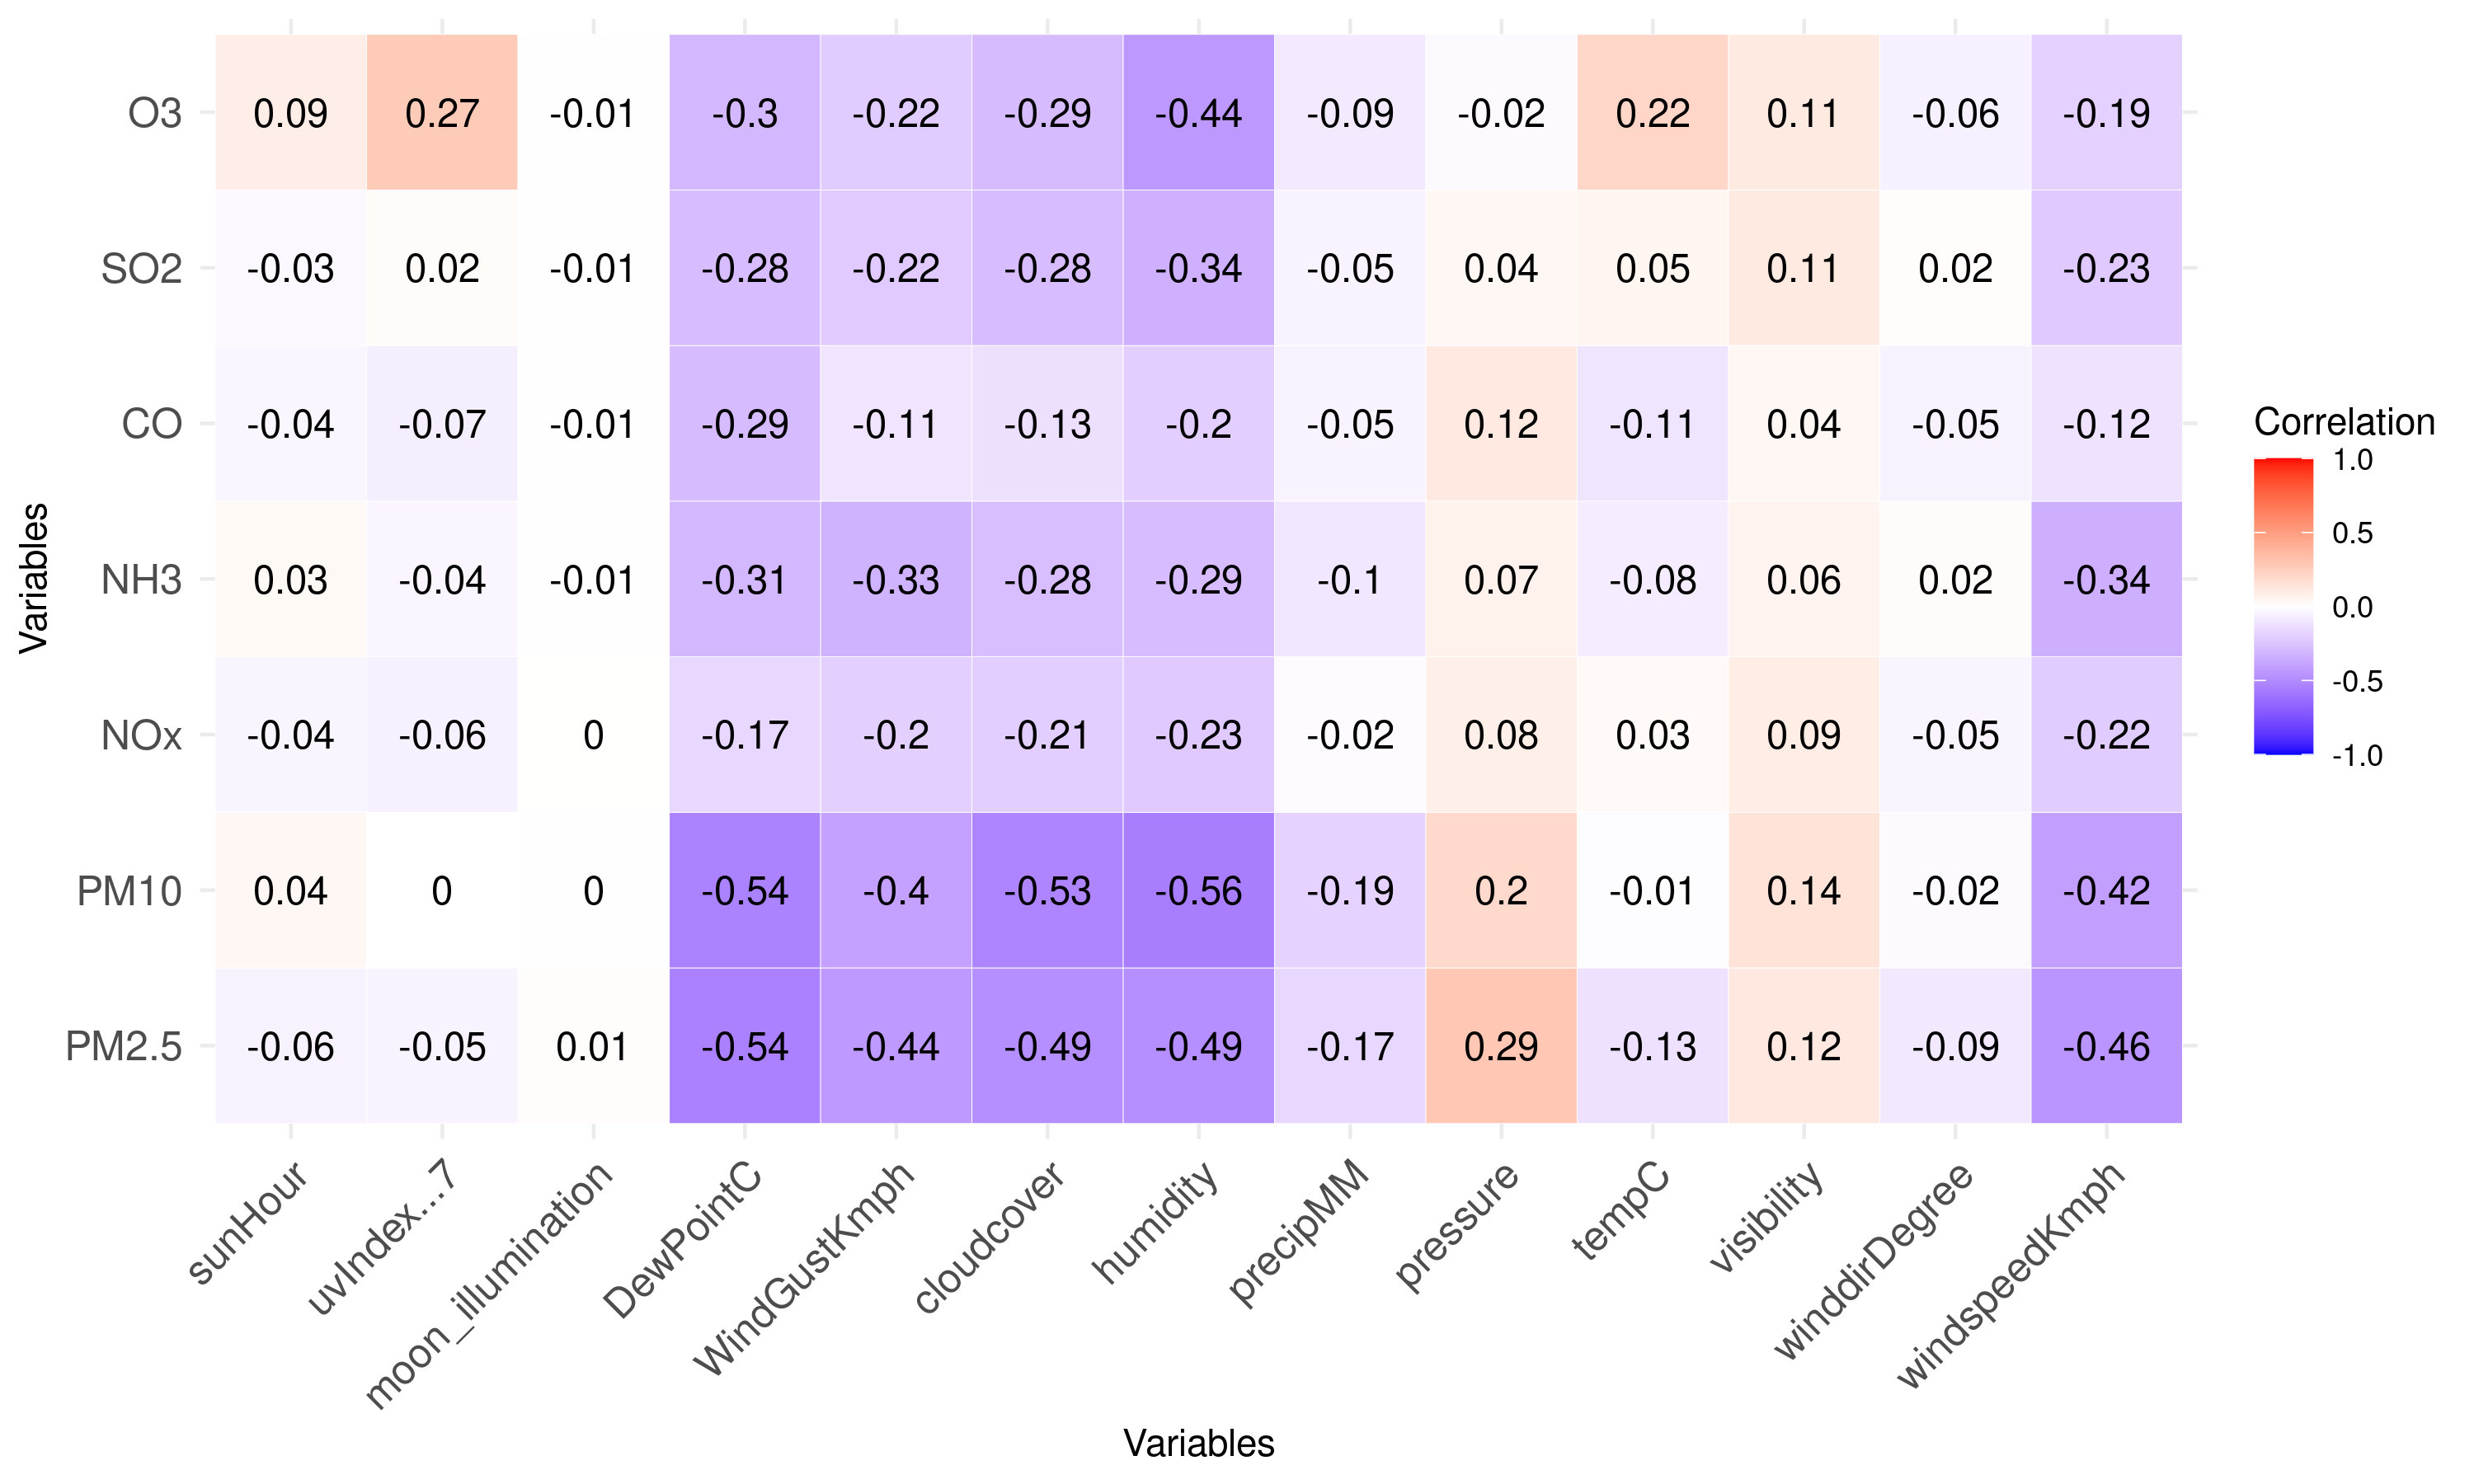
\includegraphics[width=\textwidth]{assets/feature-response-correlation.png}
  \caption{Correlation between weather features and response variables.}
  \label{fig:feature_response_correlation}
\end{figure}

The analysis revealed the following:
\begin{itemize}
    \item \textit{Humidity}, \textit{windspeed}, \textit{cloudcover}, and \textit{DewPointC} were negatively correlated with all but the CO pollutant, with the strongest correlations observed with particulate matter (\textit{PM10} and \textit{PM2.5}).
    \item \textit{O3} was also slightly positively correlated with \textit{uvIndex} and \textit{tempC}.
    \item \textit{CO} showed no notable correlation with any of the selected weather features, except a negative correlation with \textit{DewPointC}.
    \item \textit{MoonIllumination} was not correlated with any variable, as expected.
\end{itemize}

However, since this analysis relied solely on linear correlation measures, it is possible that important non-linear relationships remain undetected. To capture such relationships, several feature transformations were performed in subsequent steps.


\subsection{Feature Engineering}

Our feature engineering process focused on creating meaningful derived variables that could capture complex temporal patterns and weather-related phenomena not directly represented in the raw data. These engineered features proved to be highly effective in improving our model's predictive performance.

\subsubsection{Temporal Features}

To capture the cyclical nature of air pollution patterns, we developed several temporal features from the datetime information. First, we created a column for the hour of the day (\textit{hour\_of\_day}, ranging from 0 to 23). To properly represent the circular nature of time, we then transformed this hour variable into two continuous features using trigonometric functions: $\textit{hour\_cos} = \cos(2\pi \times \text{hour}/24)$ and $\textit{hour\_sin} = \sin(2\pi \times \text{hour}/24)$. This cyclic encoding ensures that hour 23 is correctly represented as being close to hour 0. We applied analogous transformations with a 12-hour period to create \textit{hour\_cos\_12h} and \textit{hour\_sin\_12h} features to capture any possible bi-daily patterns. Finally, we created categorical variables for the day of the week (\textit{day\_of\_week}, ranging from 1 to 7) and month of the year (\textit{month\_of\_year}, ranging from 1 to 12) to capture weekly and seasonal patterns in pollution levels. These predictors were made categorical to account for the complex seasonal patterns observed in the data.

\subsubsection{Weather-Related Features}

For weather data, we implemented several transformations. Wind direction, originally measured in degrees (0-359), was converted into two continuous features using sine and cosine transformations: $\textit{winddir\_cos} = \cos(2\pi \times \text{degree}/360)$ and $\textit{winddir\_sin} = \sin(2\pi \times \text{degree}/360)$. This cyclic encoding ensured that directions like 359° and 0° were appropriately represented as being nearly identical, which would not be the case with raw degree values.

A key feature that emerged from our literature review was the significant impact of precipitation on pollution levels during rainy seasons. To capture this effect, we developed a cumulative precipitation feature (\textit{precipMM\_24h}) that calculates the total rainfall over the previous 24 hours for each city. This feature proved to be effective in our final model, helping to capture how sustained rainfall patterns affect pollutant concentrations. Similarly, we created a 24-hour cumulative wind speed feature (\textit{windspeedKmph\_24h}) to account for the sustained impact of wind on pollutant dispersion.

Additionally, we normalized sunrise times (\textit{sunrise\_normalized}) to account for seasonal variations in daylight patterns, scaling the values between 0 and 1 to allow for better comparability across different seasons and cities. This normalization helped capture the influence of varying daylight patterns on pollution accumulation and dispersion.

These engineered features, particularly the temporal cyclic encodings and the 24-hour cumulative precipitation metric, significantly enhanced our model's ability to capture complex patterns in air pollution levels. The effectiveness of these features suggests that both the cyclic nature of pollution patterns and the sustained impact of weather conditions play crucial roles in determining air quality levels.


\newpage


% ---------------------------------------------------------------------------------------
% ---------------------------------------------------------------------------------------
% ---------------------------------------------------------------------------------------



% Acknowledgements should go at the end, before appendices and references


% Manual newpage inserted to improve layout of sample file - not
% needed in general before appendices/bibliography.

\bibliography{references}

% Note: in this sample, the section number is hard-coded in. Following
% proper LaTeX conventions, it should properly be coded as a reference:

%In this appendix we prove the following theorem from
%Section~\ref{sec:textree-generalization}:



\end{document}
